\chapter{Previous Work}
\label{sec:prevWork}

IMPORTANT: Make sure the technical/theoretical/practical issues of previous work is clearly stated.

Given a 3D CAD model of some hydraulic machinery we want to generate how things work visualizations.
Namely, adding arrows depicting the fluid movement.

The problem can be subdivided into:
\begin{enumerate}
\item \textbf{Part analysis:} Detecting fluid containers and fluid handling parts.
\item \textbf{Fluid simulation:} Simulate how the fluid behaves in the previously detected parts.
\item \textbf{Fluid visualization:} Display the fluid simulation data in a intuitive format.
\end{enumerate}

Part analysis involves two steps: part segmentation and part information extraction.
Usually 3D models consist of meshes or point clouds were there is not a clear distinction between each piece.
Consequently, any additional analysis and simulation would be overly complicated without further simplifications.  
Therefore, a segmentation stage is needed in order to divide the model into its constituent components.
Part information extraction consists of detecting the piece type, how it moves and interacts with others.
So the information saved for type would be axle, gear, reservoir, fluid conduct, etc.
In this classification parts are also organized considering fluid interaction criteria, e.g. if the piece interplays or not with the hydraulic fluid.
With respect to types of movement, it will be direction of movement, axis of rotation, axis of translation, etc.

Once the parts have been categorized and given an input force, we will have to simulate how the force is transmitted along the different elements.
In the special case where a component is a container of a fluid or is in direct contact with one, that force will have to be introduced in a fluid simulation algorithm.
The output of the simulation will then carry the information along to the next piece.

Lastly, in order to visualize the fluid simulation data we will need to generate a visual cue that will indicate intuitively the fluid movement.
Either generating arrows indicating the overall fluid movement, with an animation or showing illustrative key frames.

\section{Explanatory illustration}

Explanatory illustration has to adequately transmit motion on a still image, consequently transforming from the temporal space to the image domain.
This is usually found in comics books and instructions sets.

\subsection{Image and key frames output}

Even though comics books are regularly considered inferior forms for presenting information, each scene contains abundant data and they can be understood by children without even reading the letters.
\cite{McCloud1993} cited by \cite{Cutting2002} reviewed visualization and abstraction techniques used in comics books.
Such as, how to depict the motion of single objects and to illustrate noises and speeches bound to time.
\cite{Cutting2002} surveyed traditional techniques for depicting motion.
Including, sequences of key frames, blur, squeeze and stretch, unbalanced postures and stroboscopic effects.
The author introduced criteria to judge the effectiveness of a particular representation.
For example, evocativeness, clarity of object, direction of motion and precision of motion.

\cite{Nienhaus2005} proposed a technique to depict motion in 3D animations.
Scene and behaviour descriptions from specialized scene graphs were analysed in order to create the motion cues.
In the author's implementation the user has to select a depiction target and assign labels to it, using the graph information motion lines and simplified sketch images are generated.
\cite{Joshi2005} presented a similar approach for volumetric data.
Speedlines and flow ribbons are combined to generate illustrations encoding 3D rigid movement and flow dynamics.
The flow ribbons use comic inspired line abstraction technique to handle occlusion.
Researchers have have look into automatic illustration generation for mechanical assemblies \cite{Mitra2010}.
The author's work is based only on geometry information, extracted from 3D CAD models.
Part analysis is performed using slippage analysis, see Section \ref{SlippageAnalysis}, while the motions are extracted from an interaction graph that is defined by edge contact between the components.
The system is able to generate, motion arrows depicting mechanical assembly interaction, as well as generating key frames of periodic motions.

\subsection{Video output}

Video based illustration is applied to enhance the motion information while maintaining the original video format.
Therefore, motions are exaggerated or at the very least some hints to reinforce movement perception are added.

\cite{Collomosse2005} presented a method to embed cartoon-style motion cues in video.
Their algorithm has two stages: a motion tracking step, where a feature manually marked will be tracked; and a computer graphics stages, where a cue will be generated and added to the video.
The system can add motion lines as well as squash and stretch objects.
However, the second case is restricted to videos where the background can be reconstructed from previous frames.
\cite{Zhu2011} presented a sketching system for fluids dynamics.
The paper uses hybrid multi layered grid solver, discussed in Section~\ref{gridFluidSolvers}, to solve 2.5D fluid flow.
Flow paths and other objects can be added or changed in real time through a sketching interface.
A hydraulic graph is created and is modified behind the scenes every time the visual model is edited.
While the flow is shown using streamlines, discussed in Section~\ref{sec:flowVisualization}.
\cite{Lowe2014} showed that even though animations have become a generalized tool for visualizing dynamic systems, special care have to be taken as users can fail to extract the necessary information due to the nature of the animation.

\section{Part analysis}

Libraries of 3D mesh models are quite common \cite{Trimble2014}, \cite{GrabCAD2014}, \cite{Autodesk2014}, in addition they contain vast quantities of models.   
Usually the models are also represented using points clouds, which can be obtained easily from the meshes.
However, clouds and mesh models lack middle and high level information such as: symmetry, parallelism or part segmentation.
Therefore we must extract this information from either representation.
Since solving for general shapes is quite challenging, a number of constrained approaches have been proposed.
For a more in depth knowledge there are a number of surveys on the topic \cite{Varady1997}, \cite{Agathos2007} and \cite{Shamir2008}.

%Can divide this in region growing, wathersed, kmeans, mesh shift, shaper diameter function, random walk.
\subsection{Region growing}

Region growing algorithms start with a seed element for the sub-mesh and then perform a local greedy element addition to the current cluster.
\cite{Mizoguchi2006} proposed a mesh segmentation technique based on curvature estimation with sharp edge recognition.
The author's method performs well on mechanical objects and it is also robust to noise.
However, oversegmentation occurs in models with soft edges.
%Maybe add more papers, too lazy to do it now

%TODO Add papers on all this sections if short on words
%\subsection{Watershed}

%\subsection{Hierarchical clustering}


\subsection{Iterative clustering}

Iterative clustering is based on the k-means clustering algorithm.
Representatives for each cluster are chosen and then using some metric  the elements are assigned to the best cluster and the representatives are recalculated.
\cite{Lai2006} presented a cluster based segmentation algorithm.
The method performs better with hierarchical models composed of regions at multiple scales.
Therefore, it gives the same results regardless of model scale or the coarseness of the mesh.
A quadratic surface fitting algorithm was presented by \cite{Yan2012}.
Which combines several distance metrics to perform the quadratic minimization.

%\subsection{Mesh shift}

%\subsection{Shape diameter function}

\subsection{Random walk}

With the random walks approach, $n$ faces are chosen as seeds, with $n$ been the number of desired segments.
Then for each unlabelled face, the probabilities that a random walker will reach each labelled face are calculated.
Finally, each face is assigned to the highest probability label.
\cite{Grady2006} proposed a first random walks implementation constrained into the imaged domain.
Thereafter, \cite{Lai2009} extended it to for 3D mesh models, the author's technique also included an automatic seeding mode were seeds quantity and placement is based on a spring-like energy function.
Seeds placement can greatly affect the final segmentation.
Nevertheless, the authors tackle the issue with a post processing stage were the clusters are merged if oversegmentation occurred and the edges are smoothed.
 

\subsection{Data driven}

%Acoording to 2013 Mitra paper, this is co-analysis
\cite{Golovinskiy2009} also demonstrated a clustering technique with special emphasis on edge and face consistency.
The algorithm is based on a graph construction which encodes triangle neighbour information.
The method then performs the clustering on the graph space.
The main advantage is consistent segmentation of similar models.

\subsection{Global energy function}

\cite{DeCastro2014} presented an segmentation technique based on calculating a global discrepancy function, based on the Lambert illumination model, for each triangle in the mesh.
Then directly using that value to segment the model in several parts. 

\subsection{Hybrid}

\cite{Wang2011} approach for mesh segmentation functions with a combination of curvature estimation, Gauss mapping and B-spline surface fitting.

\subsection{Slippage analysis}
\label{SlippageAnalysis}

However all the previous methods cannot be directly applied to segment mechanical parts.
\cite{Gelfand2004} proposed a method for segmenting mechanical objects based on local slippage.
This is quite useful as it gives for each part its degrees of freedom, e.g. sphere (3 rotations), cylinder (1 rotation and 1 translation), plane (1 rotation and 2 translations), etc.
\cite{Yi2014} improved \cite{Gelfand2004} method making it more robust to noise and giving extra primitive information(e.g. normal of a plane, center of a sphere, etc).

\section{Fluid simulation}
\label{prevWorkFluidSim}

The current paradigm in fluid simulation consist of solving the Navier-Stokes equations of fluid dynamics, shown in Equations~\ref{eq:navierStokes1} and  ~\ref{eq:navierStokes1}.

\begin{gather}
\label{eq:navierStokes1}
\nabla \cdot \mathbf{u} = 0\\
\label{eq:navierStokes2}
\mathbf{u}_t = -(\mathbf{u} \cdot \nabla)\mathbf{u} + \nabla \cdot ( v \nabla \mathbf{u} - \frac{1}{\rho} \nabla p + \mathbf{f} )
\end{gather}

The first equation enforces mass conservation and ensures incompressibility, while the second encodes momentum conservation it is derived from Newton's Second Law.
Where $\mathbf{u}_t$ is the time derivative vector field of the fluid velocity, $p$  is the scalar pressure field, $\rho$ is the density of the fluid, $v$ is the kinematic viscosity and $\mathbf{f}$ represents the body force per unit mass, usually gravity.

Along the years several methods have been proposed, although all of them are based on the same Navier-Stokes equations.

\begin{itemize}
\item \textbf{Fourier Transform} techniques uses several superimposed sinusoidal waves to model the fluid behaviour.
\item \textbf{Grid} based methods track the fluid features at fixed points in space.
\item \textbf{Smooth Particle Hydrodynamics} track a large number of particle in the fluid.
\item \textbf{Hybrid} algorithms are combinations of the aforementioned methods.
\end{itemize}

Regardless of the chosen method, to update the particles in the for the next frame must be computed.
However, it is common for the algorithms to have a upper time step, if the update is computed after the limit there is no guaranty that the output would be reasonable.

Another important concept in fluid simulation is whether the simulation implements interplay within the fluid and rigid bodies that come in contact with it (solid-fluid coupling).
And how flexible is this interaction, one way solid fluid(e.g. a rock drops on a small pool of water, so the water moves but the rock is almost not affected by the  and moves it, but the fluid does not affect the rock), or fluid solid(e.g. a small buoy floating in the ocean has little effect on the surrounding water), and two way solid fluid interaction(e.g. a flexible object drops into a pool of fluid).

For more information on real time fluid simulations see \cite{Vines2012} survey.
While for survey specific to SPH fluid simulation see \cite{Ihmsen2014}.

\subsection{Fourier Transform}

When simulating fluid with periodic boundary conditions, procedural simulation can be applied with a low computational cost.
Usually this method is used with large masses of water (ocean simulation), as they are an approximation to periodic boundary conditions fluids.
The waves can be modelled as a superimposition of sinusoidal waves, which can be efficiently decomposed using Fast Fourier Transform methods \cite{Mastin1987}.
Waves produced in this fashion are visually plausible but physical accuracy is not enforced inherently by the model.

Each wave has a wave number $k$ and a wave vector $\mathbf{k}$.
\cite{Tessendorf2001} presented the basic technique in this area.
The authors modelled the ocean surface as a summation of complex sinusoids with different wave vectors.
Visually pleasing results were achieved generating random Fourier amplitudes.

The previous method was further improved by \cite{Cieutat2003}, with the addition of solid (ships, coast line, etc).
The model developed more complex wave shape and motion equations, with differentiated equations in open sea and near the shore.
And by \cite{Chiu2006} with adaptive surface tessellation.
Furthermore, the method was implemented on GPUs, and also included shallow water effects and spray dynamics.

\subsection{Grid}
\label{gridFluidSolvers}

Grid methods were among the first techniques to solve fluid simulation and so the firsts ones implement intuitive solutions.
Grid based methods solve Navier-Stokes Equations~\ref{eq:navierStokes1} and~\ref{eq:navierStokes2}, in a fixed position in space (i.e. grid).
As fluid flows, the equations are solved in each position, giving a value for speed and pressure at each time step.
This approach is advantageous as many numerical methods can be applied easily on grids and with they are more easily adaptable to GPUs implementations than other methods.

One of the firsts papers in this area introduced a Grid method \cite{Foster1996} to solve Navier-Stokes equations by applying forward Euler time integration.
However, their solid fluid coupling was one way only, the solids do not affect the fluid behaviour.
\cite{Stam1999} extended this method in order to overcome stability issues.
The author's implemented a stable solver which allowed for larger time steps, trough an operator splitting scheme and more importantly a semi-Lagrangian method to calculate the advection term.

\cite{Carlson2004} proposed solid-fluid coupling algorithm for grids models using distributed Lagrange multipliers.
Nevertheless, the author's method uses  a non adaptive grid and multiphase fluids and bubbles are not covered by it.

\subsection{Smooth Particle Hydrodynamics}

Smooth Particle Hydrodynamics(SPH) has been established as one the major breakthroughs for fluid simulations in computer graphics, positioning itself as the most popular method nowadays.
Compared to grid based methods that need high resolution grids to produce foam and splashes, SPH can achieve the same with less computational load.
Two extra advantages are that mass conservation is automatically satisfied if the amount and mass of the particles is keep constant;
and as the particles move with the fluid, the advection term does not need to be calculated explicitly.

SPH were first introduced by \cite{DesbrunMathieuandGascuel1996}, where each particle encodes its position, velocity, mass and the forces that act on it.

While, \cite{Muller2004} presented a method for computing solid fluid coupling. Where boundary particles are created on the surface of the solid and then particle coupling is calculated.
\cite{Akinci2012} further improved the previous method with the inclusion of irregular particle distributions as well as friction and dragging. 
\cite{Shao2014} also solved stability issues in the previous SPH solid-fluid coupling techniques, using a correction scheme.
Furthermore their algorithm was implemented on GPUs, thus achieving better performance than previous methods.  

\subsection{Hybrid}

Hybrid methods are combinations of the aforementioned approaches.
As with other hybrid techniques, the objective is to capitalize the advantages of each and discard the weaknesses.

A common hybrid approach is the particle-in-cell (PIC) method, \cite{Harlow1962}.
It solves the advection using SPH and the incompressibility with an Euler grid.
In more detail, the particles are averaged onto a grid where all the terms in the Navier-Stokes Equations \ref{eq:navierStokes1} and \ref{eq:navierStokes2} are calculated, except advection.
Next, the particles are translated using the grid velocity.
This method has been used in a variety of situations, for example \cite{Zhu2005} used it for sand simulation, while \cite{Horvath2009} explored fire simulations.
A further improvement is an implicit approach, namely the fluid implicit particle (FLIP) \cite{J.U.Brackbill1986}.
Where the particles are not updated directly with grid data.
The main strength of FLIP is that the advection term calculation is always stable.
However, the particles can sometimes clamp or have voids.
FLIP was extended by \cite{Raveendran2011} to be able to solve the equations in a coarse grid. 
% Instead, the variation of a quantity is computed from the grid, and this in turn is used to update particle information.

\section{Flow visualization}
\label{sec:flowVisualization}

%In each of them talk first about steady flow and then about unsteady flow 

Extensive work has been done in this area as visualizing fluid movement has a broad range of applications.
However, this is a challenging task as it has to effectively display complex and copious amounts of data.
Seeing that fluid simulation is generally solved by means of highly divided grids or with large number of particles, as explained in Section~\ref{prevWorkFluidSim}.

%TODO Changed the here option and let latex do its work, but it puts the picture before the flow visualization section
\begin{figure}
	\centering
	\begin{minipage}[t]{.45\textwidth}
		\centering
		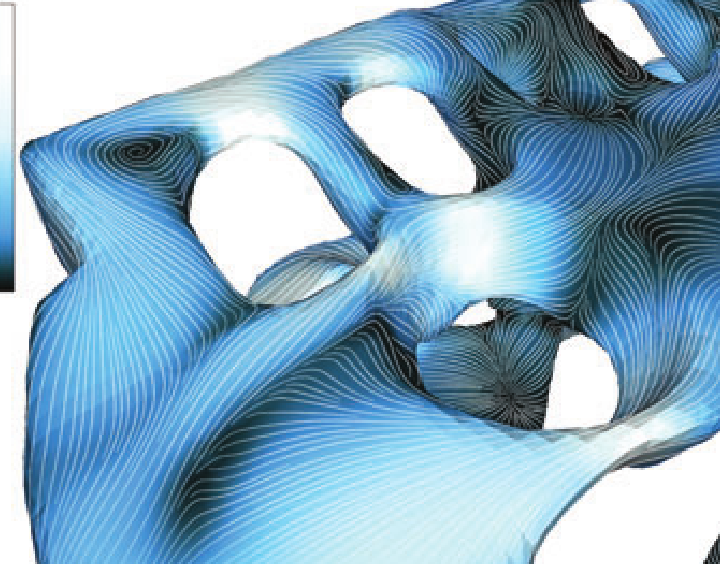
\includegraphics[width=.8\textwidth,height=4cm]{images/streamLinesSpencer}
		\caption{Streamlines on a 3D surface~\cite{Spencer2009}.}
		\label{fig:streamLines}
	\end{minipage}\hfill
	\begin{minipage}[t]{.45\textwidth}
		\centering
		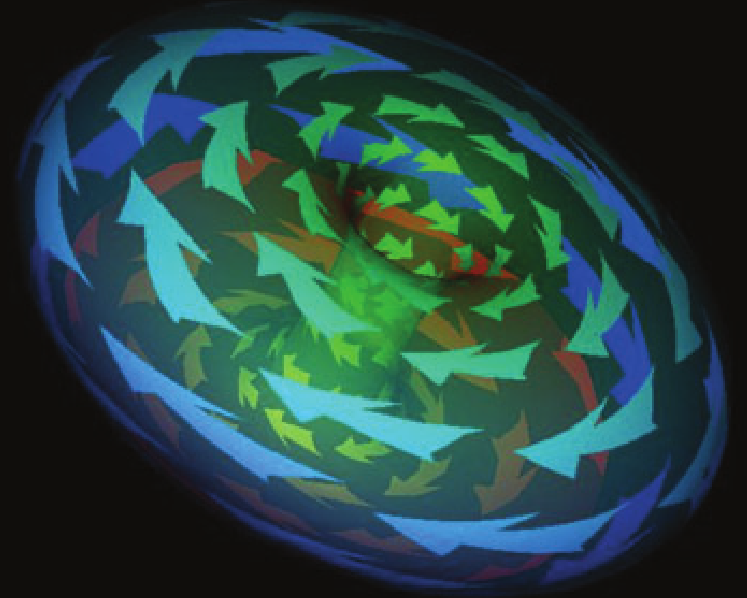
\includegraphics[width=.8\textwidth,height=4cm]{images/streamArrows}
		\caption{Arrows placed on streamlines paths in a 3D surface~\cite{loffelmann1998}.}
		\label{fig:streamArrows}
	\end{minipage}
\end{figure}

Streamlines are convenient tools to describe and visualize flow, as shown in figure~\ref{fig:streamLines}.
A streamline is defined as a curve that is everywhere tangent to flow field, i.e. it is parallel to the local velocity vector.
Therefore, they provide an intuitive mechanism to show the fluid travel direction.
Furthermore, they have properties such as: streamlines will not cross each other (flow will not go across them), or a particle in the fluid starting on one streamline will not leave it.
Once the streamlines has been calculated, instead of displaying them as such, they can be replaced by arrows arranged using some criteria.
For instance, on the path of each streamline or after clustering some streamlines together, as shown in Figure~\ref{fig:streamArrows}.

In the following sections we focus only on steady flow visualization.
For more information on the subject we refer the readers to~\cite{McLoughlin2010} survey.

\subsection{2D visualization}

On the 2D image domain, an image-guided algorithm for visualizing 2D flow in images was proposed by \cite{Turk1996}.
Which \cite{Li2008} improved, by only generating the fewest possible number of streamlines. 

\subsection{Streamlines on surfaces}

Seeding techniques for curves on 3D surfaces were explored by  \cite{Wicke2009}, who developed a technique to combine model reduction with grid based methods.
And by \cite{Spencer2009}, whose method generates streamlines only for visible parts of the surface, thus providing a significant gain in efficiency.

\subsection{Streamline rendering and placement}

Rendering too many streamlines can result in clutter and too few can lead to omit important characteristics.
There has been plenty research into optimizing streamline production and placement.
However for our hydraulic machinery the issue is less critical than in other areas.

\begin{figure}
	\centering
	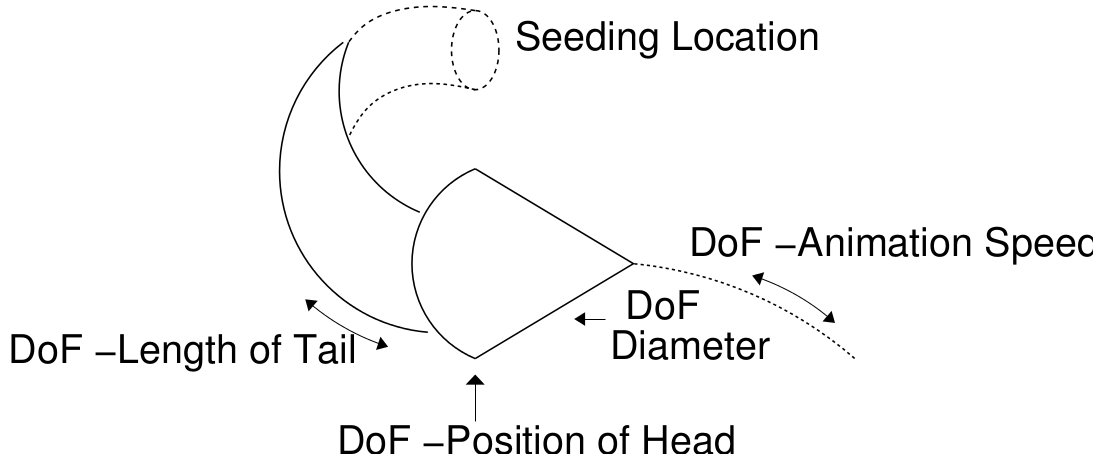
\includegraphics[scale=.2]{images/streamComet}
	\caption{Streamcomet depiction with its degrees of freedom outlined \cite{Laramee2005}.}
	\label{fig:streamComent}
\end{figure}

\cite{Laramee2005} presented the streamcomet and a fast animating technique.
A streamcomet, as shown in Figure~\ref{fig:streamComent}, is an extension of a streamline, they move along the path of a stream line, with adjustable head position, length and translucency of tail, and variable animation speed.
While the fast animating technique applies a stipple pattern to the streamline path, so the pattern is shifted at rendering time to add animation.
\cite{Rosanwo2009} proposed a dual seeding technique for streamline placement.
Dual streamlines that are orthogonal to the fluid flow are also calculated.
However they are not rendered but rather used to better decide which and how the primal streamlines are going to be drawn.
Considering the occlusion problems that normally arise in this area, \cite{Marchesin2010} tackle the streamline rendering from a view dependant perspective.
The authors precompute a random pool of streamlines.
Then, occluded areas are pruned and empty areas are reseeded for the current view via occupancy buffers.
What is more, a GPU implementation of their method is provided.
Clustering is a common technique for reducing the amount of rendered streamlines.
To address slow euclidean distance tests in clustering, \cite{McLoughlin2013} presented a signature based metric.
The streamline attributes for the signature are curvature, torsion and tortuosity.
The authors presented two variations, a fast simpler method and a hierarchical one that scarifies speed for superior results.
However, both provide a performance increase over euclidean distance calculations.

\subsection{Surface based integral objects}

Streamlines can be extended dimensionally in order to work with surfaces instead of lines, an example of a streamsurface is shown in Figure~\ref{fig:streamSurface}.
Evidently, following this path leads to more complex methods as a new dimension in added.
Nevertheless, surfaces can provide better visualization results.
For example, the use of shading gives an improved depth insight.

\begin{figure}
	\centering
	\begin{minipage}[t]{.45\textwidth}
		\centering
		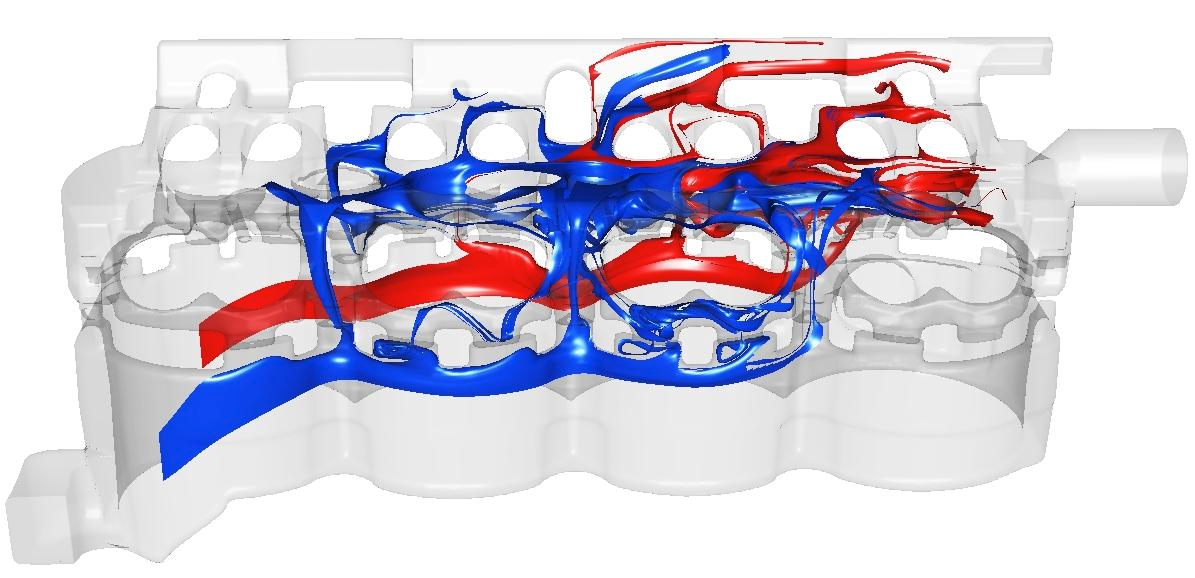
\includegraphics[width=1.05\textwidth]{images/streamSurface}
		\caption{Streamsurface illustrating fuel flow in an engine~\cite{Laramee2005a}.}
		\label{fig:streamSurface}
	\end{minipage}\qquad
	\begin{minipage}[t]{.45\textwidth}
		\centering
		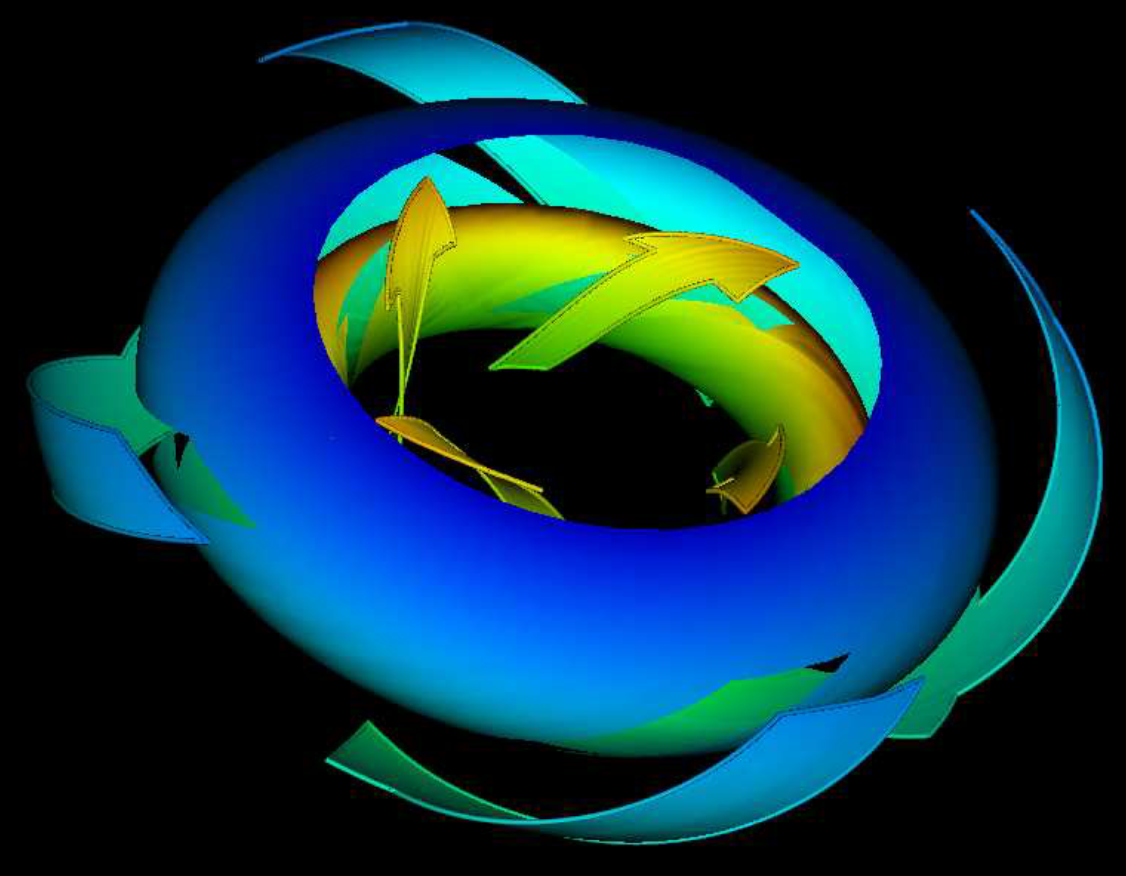
\includegraphics[width=.8\textwidth]{images/streamArrows2}
		\caption{Streamarrows in an occluded flow situation~\cite{Loffelmann1997}.}
		\label{fig:streamArrows2}
	\end{minipage}
\end{figure}

Streamsurfaces were introduced by \cite{Hultquist1992}.
The author's method seeds streamlines from a curve and those streamlines are advanced through the vector field.
New streamlines are seeded in a the points reach a certain distance.
They are also terminated if another streamline is too close.
The streamlines points are used to create the streamsurface mesh.
To aid in the interpretation of flow, \cite{Loffelmann1997} extended streamsurface model with the addition of streamarrows, as shown in Figure~\ref{fig:streamArrows}.
The author's technique involves adding arrows to show flow direction, and removing the arrow space on the surface to help with occlusion.
A hybrid method with streamlines and streamtubes was proposed by \cite{Zhang2003}.
Depicting linear anisotropy regions with streamtube and planar anisotropy ones with streamsurfaces.
The colors used for rendering encode additional anisotropy information.
More recently, \cite{Born2010} presented extensions in streamsurface rendering to address occlusion issues, as well as a GPU implementation of their technique.
Contour lines, halftoning, silhouetts, contour arrows, cuts and slabs are applied to a raw streamsurface in order to be able to depict occluded areas.

%Could be useful to talk about streamtubes.